\documentclass[10pt, colorlinks=true, urlcolor=blue]{beamer}

% Themes and colors for a professional look
\usetheme{Madrid}
\usecolortheme{seagull}
\setbeamercolor{title}{fg=white,bg=blue!80!black}
\setbeamercolor{frametitle}{fg=white,bg=blue!70!black}
\setbeamercolor{block title}{fg=white,bg=blue!80!black}
\setbeamercolor{block body}{bg=blue!5!white}
\setbeamerfont{title}{size=\fontsize{12}{16}\selectfont}

% Customize the footline layout
\setbeamertemplate{footline}
{
  \leavevmode%
  \hbox{%
    % Left field (author or custom text)
    \begin{beamercolorbox}[wd=0.25\paperwidth,ht=2.5ex,dp=1ex,center]{author in head/foot}%
      \usebeamerfont{author in head/foot}\insertshortauthor
    \end{beamercolorbox}%
    % Middle field (title)
    \begin{beamercolorbox}[wd=0.5\paperwidth,ht=2.5ex,dp=1ex,center]{title in head/foot}%
      \usebeamerfont{title in head/foot}\insertshorttitle
    \end{beamercolorbox}%
    % Right field (page number)
    \begin{beamercolorbox}[wd=0.25\paperwidth,ht=2.5ex,dp=1ex,center]{date in head/foot}%
      \usebeamerfont{date in head/foot}\insertframenumber/\inserttotalframenumber
    \end{beamercolorbox}%
  }%
}

% Set hyperlink colors
\hypersetup{
    colorlinks=true,    % Enable colored links
    urlcolor=blue,      % Color for URLs
    linkcolor=blue      % Color for internal links (optional)
}

\usepackage{minted}

\title{Python Mutability Visually Explained}
\author{Bas Terwijn}
\titlegraphic{
\includegraphics[width=0.6\textwidth]{figures/uva.png}}
\date{\today}

\begin{document}

\begin{frame}
    \titlepage
\end{frame}

\begin{frame}{Content}

  We will cover these \href{https://docs.python.org/3/reference/datamodel.html}{\texttt{Python Data Model}} topics:
  \begin{itemize}
  \item Mutability of Types
  \item Variables are References to Values
  \item Coping Values
  \end{itemize}

  \vspace{2em}
  
  These concepts are fundamental to Python programming.
  \begin{itemize}
    \item without a solid understanding you cannot avoid certain bugs
  \end{itemize}

  \vspace{2em}
  
  We will use visualization tools to help build a solid understanding:
  \begin{itemize}
  \item \href{https://pypi.org/project/memory-graph/}{\texttt{memory\_graph}}
  \item \href{https://pythontutor.com/}{\texttt{Python Tutor}}
  \end{itemize}

  \vspace{2em}

  We finish with an exercise with which you can test your understanding.
\end{frame}


\begin{frame}{Immutable and Mutable Types}
    \begin{block}{Python Types}
        Python has two distinct categories of types: Immutable, Mutable
    \end{block}

    \vspace{2em}
    
    \textbf{Immutable Types:} \texttt{bool}, \texttt{int}, \texttt{float}, \texttt{complex}, \texttt{str}, \texttt{tuple}, \texttt{bytes}, \texttt{frozenset} \\
    
    \vspace{-0.8em}
    A value of an immutable type \textbf{cannot} be changed in place. \\
    Therefore, \textbf{a} copy is made when you change it. \\
    
    \vspace{2.0em}
    
    \textbf{Mutable Types:} \texttt{list}, \texttt{set}, \texttt{dict}, \texttt{classes}, \dots (most other types) \\
    
    \vspace{-0.8em}
    A value of a mutable type \textbf{can} be changed in place. \\
    Therefore, \textbf{no} copy is made when you change it.
    
\end{frame}

\begin{frame}[fragile]
  \frametitle {Sharing Mutable Values}
  When two variable share a \textbf{mutable} value, changing one changes the other.
  \vspace{1em}
\begin{columns}
  \column{0.3\textwidth}
  \begin{minted}[fontsize=\small]{python}
           a = [4, 3, 2]
           b = a
           a += [1]
    \end{minted}
  \column{0.7\textwidth}
    \begin{center}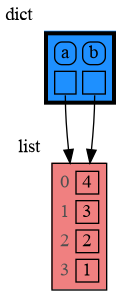
\includegraphics[width=0.25\textwidth]{figures/sharing.png}\end{center}
\end{columns}
\vspace{1em}
Sometimes we want this, but when we don't we have to \textbf{make a copy} so that each variable has its own independent value.
\end{frame}


\begin{frame}[fragile]
  \frametitle{Copying Values}
  When ``copying'' a \textbf{mutable} value, consider the amount of sharing you need:
  \vspace{-1em}
\begin{columns}
  \column{0.4\textwidth}
  \begin{minted}[fontsize=\small]{python}
      a = [[1, 2], ['x', 'y']]
      c1 = a
      c2 = copy.copy(a)
      c3 = copy.deepcopy(a)
    \end{minted}
  \column{0.6\textwidth}
    \begin{center}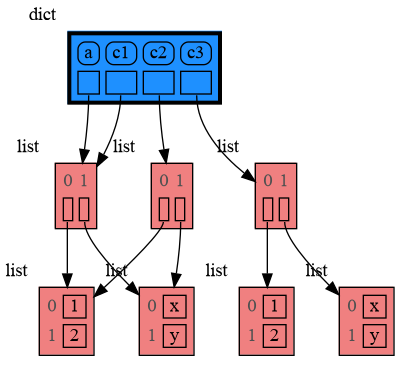
\includegraphics[width=0.7\textwidth]{figures/copy.png}\end{center}
\end{columns}
    \begin{itemize}
        \item \textbf{c1: Assignment,} nothing is copied, all the values are shared
        \item \textbf{c2: Shallow Copy,} only the value referenced by the first reference is copied, all the underlying values are shared
        \item \textbf{c3: Deep Copy,} all the values are copied, nothing is shared
        \item \ \ \, \,\, \textbf{Custom Copy,} alternatively write your own copy logic
    \end{itemize}
\end{frame}

\begin{frame}[fragile]
\frametitle{Function Calls}
  Calling a function with a \textbf{mutable} value might change that value.
  \begin{itemize}
  \item If you don't want that, make a copy.
  \end{itemize}

  \begin{columns}
    \column{0.4\textwidth}
    \begin{minted}[fontsize=\small]{python}
      def add_one(a, b, c):
         a += [1]
         b += (1,)
         c += [1]
         
      a = [4, 3, 2]
      b = (4, 3, 2)
      c = [4, 3, 2]
      add_one(a, b, c.copy())
    \end{minted}
    \column{0.6\textwidth}
    \begin{center}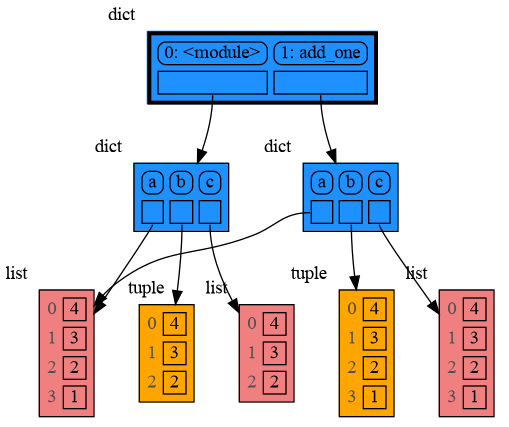
\includegraphics[width=0.9\textwidth]{figures/function_call.png}\end{center}
  \end{columns}
\end{frame}

\begin{frame}[fragile]
\frametitle{Function Calls}
  Calling a function with a \textbf{mutable} value might change that value.
  \begin{itemize}
  \item If you don't want that, make a copy.
  \end{itemize}

  \begin{columns}
    \column{0.4\textwidth}
    \begin{minted}[fontsize=\small]{python}
      def add_one(a, b, c):
         c = c.copy() # or here?
         a += [1]
         b += (1,)
         c += [1]
         
      a = [4, 3, 2]
      b = (4, 3, 2)
      c = [4, 3, 2]
      add_one(a, b, c)
    \end{minted}
    \column{0.6\textwidth}
    \begin{center}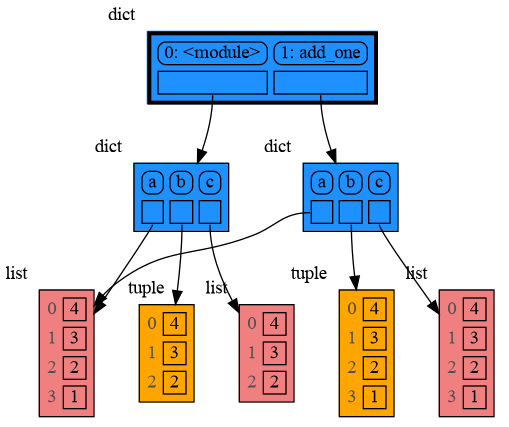
\includegraphics[width=0.9\textwidth]{figures/function_call.png}\end{center}
  \end{columns}
\end{frame}


\begin{frame}{memory\_graph Debugger Setup}
  \vspace{-1em}
  memory\_graph Debugger Setup:
  \begin{itemize}
  \item install \href{https://pypi.org/project/memory-graph/}{\texttt{memory\_graph}} and \href{https://graphviz.org/download/}{\texttt{Graphviz}}
  \item open Python source file in Visual Studio Code
  \item add line: \\ \ \ \ {\footnotesize \mintinline{python}{import memory_graph as mg}}
  \item set a breakpoint and start the debugger
  \item add watch: \\ \ \ \ {\footnotesize \mintinline{python}{mg.render(mg.get_call_stack_vscode(), 'my_graph.pdf')}}
  \item manually open file ``my\_graph.pdf'', resize window,  and set 'Always on Top'
  \end{itemize}
  
  \vspace{2em}
  
  Problem with Adobe Acrobat Reader that blocks updates to the PDF file:
  \begin{itemize}
  \item install non-blocking PDF reader as your 'Default PDF Reader': \\ \ \ \ Evince, Okular, SumatraPDF, ...
  \item or add watch: \\ \ \ \ {\footnotesize \mintinline{python}{mg.render(mg.get_call_stack_vscode(), 'my_graph.png')}}
  \end{itemize}
\end{frame}

\begin{frame}[fragile]\frametitle{memory\_graph Non-Debugger Setup}
  memory\_graph Non-Debugger Setup:
  \begin{itemize}
  \item install \href{https://pypi.org/project/memory-graph/}{\texttt{memory\_graph}} and \href{https://graphviz.org/download/}{\texttt{Graphviz}}
  \item open Python source file in any editor
  \item add line: \\ \ \ \ {\footnotesize \mintinline{python}{import memory_graph as mg}}
  \item add line where you want to graph: \\
    \ \ \ {\footnotesize \mintinline{python}{mg.show(mg.get_call_stack())}}\\
    \ \ \ {\footnotesize \mintinline{python}{mg.render(mg.get_call_stack(), 'my_graph.png')}}\\
  \item add parameter to block for \texttt{<Enter>} key press:\\
    \ \ \ {\footnotesize \mintinline{python}{block=True}}
  \item see \href{https://pypi.org/project/memory-graph/}{\texttt{memory\_graph}} docs for examples
  \end{itemize}

  \vspace{2em}
  
  Aliases:
 \begin{minted}[fontsize=\small]{python}
   from memory_graph import d, ds
   d()  # mg.show(locals(), block=True)
   ds() # mg.show(mg.get_call_stack(), block=True)
 \end{minted}
\end{frame}


\begin{frame}{Python Tutor}
  \href{https://pythontutor.com/}{\texttt{Python Tutor}}\\ 
  Philip J. Guo, Associate Professor of Cognitive Science, University of California\\
  \vspace{1em}\\
  Pros:
  \begin{itemize}
  \item no installation or setup required
  \item widely known
  \item supports multiple programming languages
  \item can debug backwards
  \item good graph stability over time
  \end{itemize}
  Cons: (\href{https://docs.google.com/document/d/13_Bc-l2FKMgwPx4dZb0sv7eMfYMHhRVgBRShha8kgbU/}{\texttt{Python Tutor Limitations}})
  \begin{itemize}
  \item runs single file in a webbrower
  \item limited program: size, runtime, memory usage
  \item can only import standard library modules
  \item no reading/writing files or command-line arguments
  \end{itemize}
\end{frame}

\begin{frame}{Example: Recursion}
  factorial
  power\_set
\end{frame}

\begin{frame}{Exercise}
  mental model
\end{frame}


\end{document}
